\subsection{Conversion: Teacher requests and the student's responsiveness}
\label{sec:local}\label{sec:motif-attenuated}\label{sec:response}\label{sec:modes}
\label{sec:conversion}\label{sec:conversion:geometry}

\leavevmode

\begin{wrapfigure}{r}{.44\textwidth}
\vspace{-9pt}
\centering
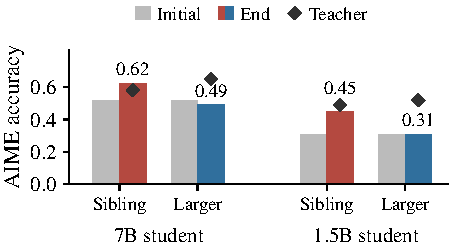
\includegraphics[width=\linewidth]{figures/section42/benchmark.pdf}
\caption{Initial/end AIME accuracy; diamonds mark teachers. Red: sibling-taught; blue: larger-teacher taught.}
\label{fig:conversion-bench}\label{fig:hook}
\vspace{-8pt}
\end{wrapfigure}

\noindent\textbf{A strong teacher can transfer little.}\quad
We open with an intriguing empirical puzzle identified in the OPD community \citep{rethinking_opd_2026}: a larger (same-family) teacher can transfer less than an RL-trained sibling even when they are nearly matched in bechmark performance, and \citet{rethinking_opd_2026} suggests cancellation among token-level gradient signals as a possible explanation. We revisit this comparison at 1.5B and 7B (\cref{fig:conversion-bench}), holding the starting DeepSeek-R1-Distill-Qwen student and OPD recipe fixed within each scale. JustRL-1.5B and AceReason-Nemotron-7B yield substantial gains, whereas the larger DeepSeek-7B and DeepSeek-14B teachers transfer little throughout training despite higher benchmark scores (\cref{app:collective-protocol}). We call these runs \emph{healthy} and \emph{stalled}. We find that the teachers' request fields differ substantially in semantic functions, and that the student's responsiveness to these requests separates in two axes: coherence of the gradient signals, and kernel adaptation toward the requests. Along the way, we develop \emph{early-training diagnostics} that help reveal the ``request-conversion'' health of a training run.

\begin{figure}[!h]
\centering
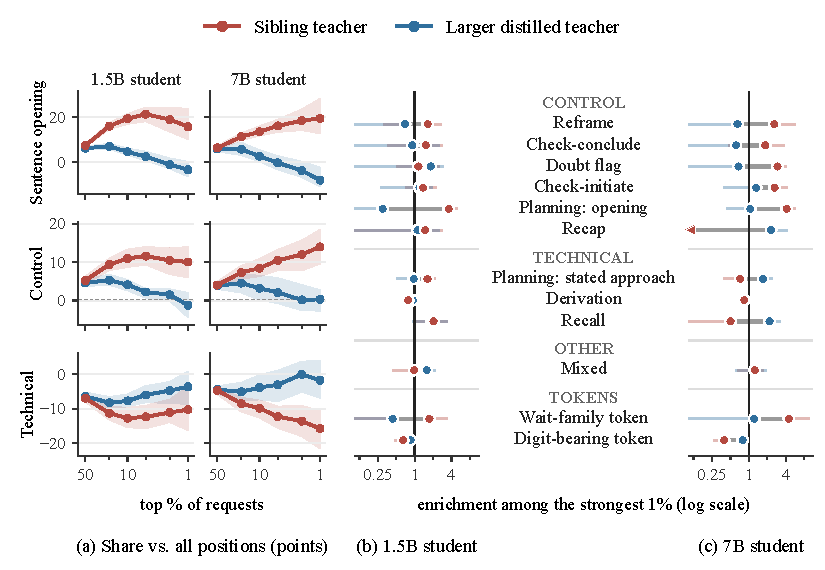
\includegraphics[width=0.85\linewidth]{figures/section42/fig_request_fields.pdf}
\caption{\textbf{Teacher request fields differ systematically.}
In (a), each curve shows how much more (or less) often a semantic or token-position class appears among a teacher's top 50\%, 20\%, \ldots, 1\% of requests than among all annotated positions, in percentage points (so 0 = no preference). The RL-sibling teachers' increasingly emphasize requests on sentence openings and ``control-oriented'' moves, while the larger teachers' stay in sentence interiors and ``technical-oriented'' content. In (b) we show finer semantic categories of the request fields. Each dumbbell pairs the teachers' enrichment among their $1\%$ largest-normed of initial requests. $1$ denotes corpus-level prevalence. See \cref{app:collective-types} for finer details on the classes and how we conduct the interpretability analysis.}
\label{fig:conversion-tokens}
\end{figure}

\paragraph{How do the request fields differ?} As we see in the OPD update loop in \cref{sec:loop}, the teacher's request population $\Gamma_t$ at time 0 ``kickstart'' the whole learning process, from which the shared-parameter student model propagates into policy motion via its kernel $K_t$. Since the student starts out to be the same while the teachers are different across the healthy and stalled runs, their request fields become the natural entry point for our analysis.

On fixed initial-student rollouts, \cref{fig:conversion-tokens} compares where each teacher's largest-normed requests occur. (a) shows the coarse tendencies of the semantics of the requests as we move up the request-norm percentile, while (b) and (c) show the finer semantic categories and contrast the teachers' distinct request fields. We find that the RL-sibling teachers increasingly emphasize reasoning-management and initiating positions, while the larger teachers place relatively more of their strongest requests at technically oriented (e.g. digit-bearing, recalling mathematical fact) positions. This separation connects to findings in the reasoning-interpretability community, that RL tends to improve how well the model ``orchestrates'' the base reasoning mechanisms (including epistemic control abilities) \citep{venhoff2025base}. Full setup and analysis results are in \cref{app:collective-types}.



\paragraph{From requests to motion.}
Figure \ref{fig:conversion-tokens} shows that the healthy and stalled teachers provide systematically different request fields in the large-normed stratum, but this alone does not help us understand which teacher's request field converts better into policy motion along along the request field. 
Recall that for a prefix population $\nu$, the gradient is $g_t(s)=\Phi_t(s)^\top B_t(s)$ in terms of the tangent map and the request, $u_t=\Ex_\nu g_t(s)$ the average gradient, and $P_t=\Ex_\nu\|B_t(s)\|^2$ the request norm, or ``pressure'' (recall $B$ is the request field induced by the teacher-student disagreement).
Under gradient flow $\dot\theta_t=u_t$, the \emph{coefficient of the logit response $\dot{z}_t$ along the request field $B_t$ on $\nu$} can be written as
\begin{equation}
\Xi_t[B_t]
=\frac{\langle B_t,\dot z_t\rangle_\nu}{P_t}
=\frac{\|u_t\|^2}{P_t},
\qquad
\dot z_t=\Xi_t[B_t]B_t+r_t,\quad
\langle B_t,r_t\rangle_\nu=0,
\label{eq:collective-response}
\end{equation}
where we define the distribution-level inner product $\langle F,G\rangle_\nu=\Ex_\nu[F^\top G]$ and $P_t>0$. With nonzero denominators, this \emph{collective conversion gain} factors as

\begin{equation}
\Xi[B]=
\underbrace{\frac{\Ex_{s\sim\nu}\|\Phi(s)^\top B(s)\|^2}{P}}_{\text{accessibility }A}
\underbrace{\frac{\|\Ex_{s\sim\nu} g(s)\|^2}{\Ex_{s\sim\nu}\|g(s)\|^2}}_{\text{coherence }C},
\qquad \|u\|^2=P\Xi=PAC.
\label{eq:pac}
\end{equation}
\emph{Accessibility} averages the self-kernel Rayleigh coefficients $B(s)^\top K(s,s)B(s)/\|B(s)\|^2$, weighted by request energy: it measures how \emph{responsive} the student's tangent map $\Phi(s)$ is to the requests $B(s)$. Coherence measures how well the resulting parameter updates $g(s)=\Phi(s)^\top B(s)$ combine: aligned updates reinforce one another, while cancellation lowers $C$. Thus ``conversion'' of requests into parameter-update-induced policy motion not only depend on pressure $\Ex_\nu\|B_t(s)\|^2$, but even if two runs have similar gradient norm with high pressure, the requests need not convert efficiently due to low accessibility (poor parameter-level motion per unit request norm at a prefix) or coherence (poor cross-prefix aggregation of parameter motion). The deeper geometric interpretations and derivations are in \cref{app:collective-proof}. We now examine what the actual training runs reveal.

\paragraph{Coherence contrasts at 7B.}
At 7B, healthy requests have near equal accessibility as the stalled requests but $2.75$--$3.24\times$ higher coherence, yielding $2.27$--$2.62\times$ higher collective gain $\Xi$ across the two sampled high-strength strata (\cref{fig:conversion-initial}). Therefore, even though the gradient norms across the healthy and stalled runs are similar, we see that it is the greater pressure in the stalled run which masks the weaker coherence of the update forces for the stalled run. For this 7B case, the gradient-incoherence conjecture in \citet{rethinking_opd_2026} is corroborated.

\begin{figure}[!h]
\centering
\begin{subfigure}[t]{.35\linewidth}
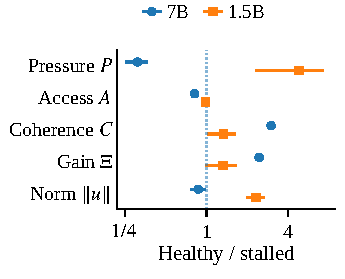
\includegraphics[width=\linewidth]{figures/section42/initial_gain_revised.pdf}
\caption{Initial conversion.}
\label{fig:conversion-initial}
\end{subfigure}\hfill
\begin{subfigure}[t]{.32\linewidth}
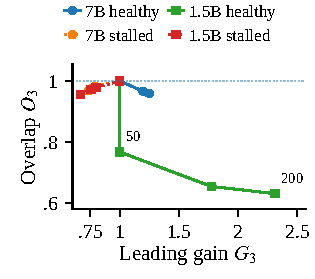
\includegraphics[width=\linewidth]{figures/section42/eigenframe_revised.pdf}
\caption{Amplification and reorientation.}
\label{fig:conversion-geometry}
\end{subfigure}\hfill
\begin{subfigure}[t]{.30\linewidth}
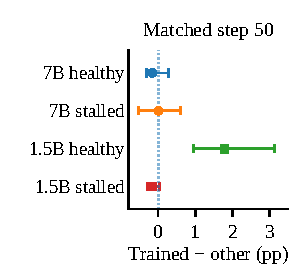
\includegraphics[width=\linewidth]{figures/section42/specificity_revised.pdf}
\caption{Teacher-relative reorientation.}
\label{fig:conversion-turn}
\end{subfigure}
\caption{\textbf{Collective conversion and acquired responsiveness distinguish the pairings.} (a) Healthy/stalled ratios; segments show the range across the \textsc{control} and \textsc{technical} strata. (b) Median leading-three eigenvalue gain $G_3$ and eigen-subspace overlap $O_3$. (c) Step-50 paired trained-minus-other-field projection gain. Definitions and full results are in \cref{app:collective-geometry,app:collective-specificity}.}
\label{fig:collective-dynamics}\label{fig:absorb}
\end{figure}

\paragraph{Evolving accessibility contrasts at 1.5B.}
At 1.5B the mechanism is richer: \emph{initial} accessibility is similar and coherence differs less; while we do see greater pressure for the healthy run (roughly $2$--$2.7\times$, which yields larger gradient norm), conversion of the requests at time 0 contrasts less across the two runs. This motivates examining how responsiveness \emph{evolves} as the student learns.



First, we note that live accessibility changes with \emph{both} the request $B_t$ and the kernel $K_t$, for instance, in a healthy run, $B_t$ can deplete learnable components and rotate away from the student's tangent map. To isolate kernel motion and how accessibility changes, we freeze each teacher's initial field $B_0$, prefix bank, and token coordinates, then reapply the same request field at every checkpoint\footnote{Time-$0$ request field is the least confounded as the initial student is the same in both the healthy and stalled runs. In practice, any representative probe bank of prefixes can be used to examine, for instance, the conversion health of more specific reasoning behaviors.}. The common initialization anchors both fields to the same student, while preserving their distinct request profiles we saw earlier with the different teachers. With $b_0(s)=B_0(s)/\|B_0(s)\|$,
$a_t(s)=b_0(s)^\top K_t(s,s)b_0(s)
       =\sum_j\lambda_{j,t}(s)|v_{j,t}(s)^\top b_0(s)|^2.
$
Here $(\lambda_{j,t},v_{j,t})$ are eigenpairs (eigenvalues and eigenvectors) of the self-kernel $K_t(s,s)$, and the request-energy-weighted average of $a_t(s)$ is $A_t[B_0]$. Larger eigenvalues amplify accessible directions; turning strong eigendirections toward $B_0$ makes more of the same request visible. Both can increase local responsiveness (\cref{app:collective-frozen}).



At 1.5B in the healthy run, leading-subspace overlap falls to $0.77$ by step 50 while leading strength remains near its initial value (\cref{fig:conversion-geometry}). This means its eigenframe \emph{re-orients towards the request field} in the early phase of training with nearly no scaling-amplification in the leading eigenvectors: the fixed request gains a median $5.5$ percentage points of top-three projection, and its paired gain exceeds the other teacher's by $1.79$ points (\cref{fig:conversion-turn}). 
By step 200, leading eigenvalue strength reaches $2.31\times$ and median request-direction sensitivity $2.08\times$ the baseline. In contrast, the stalled run \emph{contracts} in leading eigenvalue strengths and sensitivity ($0.67\times$ and $0.83\times$ respectively). 
At 7B in the healthy run, eigenvector rotation is much less pronounced and adaptation is primarily amplification of the existing eigenframe: leading strength reaches $1.25\times$ with overlap $0.96$ against the initial frame, while stalled leading strength falls to $0.74\times$.

These results distinguish healthy and stalled pairings \emph{early on} in an OPD training run in the requests they receive and the responsiveness their tangent geometry develop, giving diagnostics beyond the standard gradient norm and training loss from the request-conversion aspect. The next sub-section will study what comes next: when there is significant policy motion, cumulated over time, where do they head to? Why do two student models OPD-trained under the same teacher, both reducing training loss substantially, have different generalization performance under OPD?
